\subsection{Overview of different numerical methods}
\begin{frame}{Numerical methods}

5 different numerical schemes tested:
\begin{itemize}
  	\item TVDLF
  	\item  HLL
  	\item HLLC
  	\item TVD-MUSCL 
  	\item FD
\end{itemize}

\end{frame}



\begin{frame}{TVDLF - Total Variation Diminishing (TVD) concept}
	Total variation of numerical approximation of u:
	\begin{equation*}
		TV(u^n) = \sum_{i=0}^{N} |u_{i+1}^n-u_i^n|
	\end{equation*}
	Scheme is total variation diminishing in time if
	\begin{equation*}
		TV(u^{n+1}) \leq TV(u^{n}) \; \; \; \forall n
	\end{equation*}
\end{frame}


\begin{frame}{TVDLF}
	First order Lax-Friedrichs scheme:
	\begin{equation*}
		U_j^{n+1} = U_j^n - \frac{\Delta t}{\Delta x} \left( F_{j+1/2} - F_{j-1/2} \right) + \frac{1}{2} \left( \Phi_{j+1/2} - \Phi_{j-1/2} \right)
	\end{equation*}
	where
	\begin{equation*}
		F_{j+1/2} = \frac{F_j + F_{j+1}}{2}
	\end{equation*}
	\begin{equation*}
		\Phi_{j+1/2} = U_{j+1}-U_j
	\end{equation*}
	Scheme is TVD $\Leftrightarrow$ CFL condition satisfied \newline
	Scheme is first order accurate \newline
	Reduce numerical diffusion (with local Courant number, maximal speed):
	\begin{equation*}
		\Phi_{j+1/2} = \frac{\Delta t}{\Delta x} c_{j+1/2}^{max} \left( U_{j+1}-U_j \right)
	\end{equation*}
\end{frame}
	
	
\begin{frame}{TVDLF - second order spatial accuracy}
	Linear approximation of U and fluxes at boundary interfaces \newline
	U at $x_{j+1/2}$, linear interpolation:
	\begin{equation*}
		U_{j+1/2}^L = U_j^n + \frac{1}{2} \bar{\Delta U}_j^n
	\end{equation*}
	\begin{equation*}
		U_{j+1/2}^R = U_{j+1}^n - \frac{1}{2} \bar{\Delta U}_{j+1}^n
	\end{equation*}
	Limited slopes $\bar{\Delta U}$ will be defined later
	\begin{equation*}
		F_{j+1/2} = \frac{F(U_{j+1/2}^L) + F(U_{j+1/2}^R)}{2}
	\end{equation*}
	\begin{equation*}
		\Phi_{j+1/2} = \frac{\Delta t}{\Delta x} c_{j+1/2}^{max} \left( U_{j+1/2}^R-U_{j+1/2}^L \right)
	\end{equation*}
\end{frame}

\begin{frame}{TVDLF - slope limiter}
	Required to ensure TVD property \newline
	For example \textit{minmod} limiter
	\begin{equation*}
	\bar{\Delta U}_j = minmod(\Delta U_{j-1/2},\Delta U_{j+1/2})
	\end{equation*}
	with
	\begin{equation*}
		\Delta U_{j+1/2} = U_{j+1} - U_j
	\end{equation*}
	and
	\begin{equation*}
		minmod(w_1,w_2,\ldots,w_n) = 
	\end{equation*}
	\begin{equation*}
		sgn(w_1) max [0,min(|w_1|,sgn(w1)w_2,\ldots,sgn(w_1)w_n)]
	\end{equation*}	
	The \textit{minmod} function takes the argument with the smallest modulus when all arguments have the same signs and otherwise it is zero.
\end{frame}

\begin{frame}{TVDLF - Temporally second order accuracy}
	Use Hancock's predictor step:
	\begin{equation*}
		U_j^{n+1/2} = U_j^n - \frac{1}{2} \frac{\Delta t}{\Delta x} \left[ F(U_j^n+\frac{1}{2} \bar{\Delta U}_j^n) - F(U_j^n-\frac{1}{2} \bar{\Delta U}_j^n) \right]
	\end{equation*}
	used for calculating linear extrapolations:
	\begin{equation*}
	U_{j+1/2}^L = U_j^{n+1/2} + \frac{1}{2} \bar{\Delta U}_j^n
	\end{equation*}
	\begin{equation*}
	U_{j+1/2}^R = U_{j+1}^{n+1/2} - \frac{1}{2} \bar{\Delta U}_{j+1}^n
	\end{equation*}
\end{frame}

\begin{frame}{TVD-MUSCL}
MUSCL = Monotonic Upstream Scheme for Conservation Laws 
\begin{itemize}
	\item same Hancock predictor step and upwinding as TVDLF
	\item upwinding is applied for characteristic variables rather than conservative variables
\end{itemize}
Characteristic variables $\vec{r}^k$
\begin{itemize}
	\item linear combinations of conservative variables
	\item right eigenvectors of $\partial \vec{F} / \partial \vec{U}$
	\begin{equation*}
	\frac{\partial \vec{F}}{\partial \vec{U}} \vec{r}^k = c^k \vec{r}^k
	\end{equation*}
	\item eigenvalues $c^k$ are real
	\item eigenvectors form a complete orthogonal basis
	\item left eigenvectors $\vec{l}^k$:
	\begin{equation*}
	\vec{l}^k \cdot \vec{r}^k = \delta_{k,m}
	\end{equation*}
\end{itemize}
\end{frame}

\begin{frame}{TVD-MUSCL}
	Modify $\vec{\Phi}$:
	\begin{equation*}
	\vec{\Phi} = \frac{\Delta t}{\Delta x} \sum_{k} \vec{r}^k | c^k | \vec{l}^k \cdot (\vec{U^R} - \vec{U^L})
	\end{equation*}
	where $\vec{r}^k$, $c^k$ and $\vec{l}^k$ are calculated for $U_{j+1/2}$
	\begin{itemize}
		\item $\vec{l}^k \cdot (\vec{U^R} - \vec{U^L})$ determines jump in k-th characteristic variable
		\item multiplication by $\vec{r}^k$ transforms result back to conservation variables
	\end{itemize}
	Comparison to TVDLF
	\begin{itemize}
		\item Advantage: use of eigenvalue $c^k$ instead of largest eigenvalue $c^{max}$ $\Rightarrow$ upwinding is accurate for each characteristic variable $\Rightarrow$ less numerical diffusion
		\item Disadvantage: left and right eigenvectors must be calculated for each cell interface (can be very expensive)
	\end{itemize}
\end{frame}



\begin{frame}{FD}
	Finite Differences \newline
	The flow variables are given as point-wise values $U_j$ at locations $x_j$ as:
	\begin{equation*}
	U_j(t) = U(x_j,t)
	\end{equation*}
	Difference formulae of a given order of accuracy can be derived from Taylor expansion around the grid points \newline
	
\end{frame}

\begin{frame}{FD}
	Example, 1D, grid spacing $\Delta x$: \newline
	$\rightarrow$ a first order spatial derivative can be approximated by the centered finite difference formula:
	\begin{equation*}
	\frac{U_{j+1}-U_{j-1}}{2 \Delta x} 
	\end{equation*}
	\begin{equation*}
	= \frac{1}{2 \Delta x} \left[ U_j + \Delta x \partial_x U + \frac{(\Delta x)^2}{2!} \partial_{xx} U + \ldots	 \right]	
	\end{equation*}
	\begin{equation*}
	- 	\frac{1}{2 \Delta x} \left[ U_j - \Delta x \partial_x U + \frac{(\Delta x)^2}{2!} \partial_{xx} U + \ldots	 \right] 
	\end{equation*}
	\begin{equation*}
	= \partial_x U + O((\Delta x)^2)
	\end{equation*}
\end{frame}


\begin{frame}{HLL}
	Riemann solver of Harten, Lax and van Leer \newline
	System of one-dimensional conservation laws:
	\begin{equation*}
	q_t + f(q)_x = 0
	\end{equation*}
	with
	\begin{equation*}
	q(x,0) = \left\{ \begin{matrix} q_l & if \; x < 0 \\ q_r & if \; x > 0 \end{matrix}\right.
	\end{equation*}
\end{frame}

	
\begin{frame}		
\begin{figure}
\centering
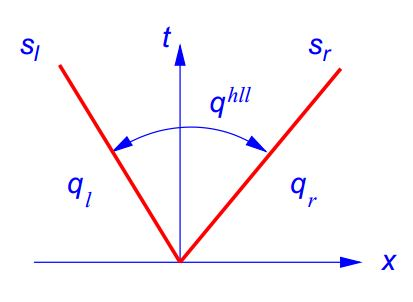
\includegraphics[width=0.9\linewidth]{../../figs/hll_fig}
\label{fig:hll_fig}
\end{figure}
\end{frame}

\begin{frame}{HLL}
	Integrating over control volume:
	\begin{equation*}
	q^{hll} = \frac{s_r q_r - s_l q_l + f_l - f_r}{s_r-s_l}
	\end{equation*}	
	Following approximation is proposed:
	\begin{equation*}
	\tilde{q}(x,t) = \left\{ \begin{matrix} q_l & if \; \frac{x}{t} \leq s_l \\ q^{hll} & if \;  s_l \leq \frac{x}{t} \leq s_r \\ q_r & if \; \frac{x}{t} \geq s_r \end{matrix}\right.
	\end{equation*}
	Corresponding flux:
	\begin{equation*}
	f_{i+1/2}^{hll} = \left\{ \begin{matrix} f_l & if \; 0 \leq s_l \\ \frac{s_r f_l - s_l f_r + s_l s_r (q_r - q_l)}{s_r - s_l}	 & if \;  s_l \leq 0 \leq s_r \\ f_r & if \; 0 \geq s_r \end{matrix}\right.
	\end{equation*}
\end{frame}

\begin{frame}{HLL}
	These formulas can be used in the explicit conservative formula:
	\begin{equation*}
	q_i^{n+1} = q_i^n + \frac{\Delta t}{\Delta x} \left[ f_{i-1/2} - f_{i+1/2} \right]
	\end{equation*}	
	Wave speeds $s_l$ and $s_r$ must be estimated.
\end{frame}

\begin{frame}{HLLC}
	Modification of HLL scheme in which the missing contact and shear waves are restored.
	
\begin{figure}
\centering
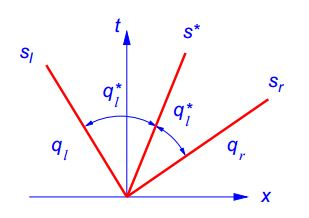
\includegraphics[width=0.7\linewidth]{../../figs/hllc_fig}
\label{fig:hllc_fig}
\end{figure}
\end{frame}

\begin{frame}{HLLC}
	\begin{equation*}
	\tilde{q}(x,t) = \left\{ \begin{matrix} q_l & if \; \frac{x}{t} \leq s_l \\ q_l^{*} & if \;  s_l \leq \frac{x}{t} \leq s^{*} \\ q_r^{*} & if \; s^{*} \leq \frac{x}{t} \leq s_r \\ q_r & if \; \frac{x}{t} \geq s_r \end{matrix}\right.
	\end{equation*}
	\begin{equation*}
	f_{i+1/2}^{hllc} = \left\{ \begin{matrix} f_l & if \; 0 \leq s_l \\ f_l + s_l (q_l^{*}-q_l) & if \;  s_l \leq 0 \leq s^{*} \\ f_r + s_r (q_r^{*}-q_r) & if \; s^{*} \leq 0 \leq s_r \\ f_r & if \; 0 \geq s_r \end{matrix}\right.
	\end{equation*}
	Intermediate states $q_l^{*}$ and $q_r^{*}$ can be determined. \newline
	Wave speeds $s_l$, $s_r$ and $s^{*}$ need to be estimated.
\end{frame}



